
%(BEGIN_QUESTION)
% Copyright 2006, Tony R. Kuphaldt, released under the Creative Commons Attribution License (v 1.0)
% This means you may do almost anything with this work of mine, so long as you give me proper credit

Determine what will happen at the following steps in the sequence (when prompted for a response) in this pressure transmitter calibration setup:

$$\includegraphics[width=15.5cm]{i00463x01.eps}$$

\begin{itemize}
\item{} {\bf Step 1:} Open valves 1 and 2
\vskip 5pt
\item{} {\bf Step 2:} Close valves 3 and 4
\vskip 5pt
\item{} {\bf Step 3:} Operate hand pump until manometer registers maximum pressure
\vskip 5pt
\item{} {\bf Step 4: (4 points)} Quickly open and close valve 4 -- {\it does the manometer indication drop greatly, slightly, or not at all?}
\vskip 5pt
\item{} {\bf Step 5:} Close valve 2
\vskip 5pt
\item{} {\bf Step 6: (4 points)} Quickly open and close valve 4 -- {\it does the manometer indication drop greatly, slightly, or not at all?}
\vskip 5pt
\item{} {\bf Step 7:} Close valve 1
\vskip 5pt
\item{} {\bf Step 8: (4 points)} Quickly open and close valve 3 -- {\it does the manometer indication drop greatly, slightly, or not at all?}
\end{itemize}

\underbar{file i00463}
%(END_QUESTION)





%(BEGIN_ANSWER)

\begin{itemize}
\item{} {\bf Step 4:} Quickly open and close valve 4 -- manometer indication drops {\bf slightly}
\item{} {\bf Step 6:} Quickly open and close valve 4 -- manometer indication {\bf does not drop} at all
\item{} {\bf Step 8:} Quickly open and close valve 3 -- manometer indication drops {\bf greatly}
\end{itemize}

%(END_ANSWER)





%(BEGIN_NOTES)

\vskip 20pt \vbox{\hrule \hbox{\strut \vrule{} {\bf Virtual Troubleshooting} \vrule} \hrule}

This question is a good candidate for a ``Virtual Troubleshooting'' exercise.  Presenting the diagram to students, you first imagine in your own mind a particular fault in the system.  Then, you present one or more symptoms of that fault (something noticeable by an operator or other user of the system).  Students then propose various diagnostic tests to perform on this system to identify the nature and location of the fault, as though they were technicians trying to troubleshoot the problem.  Your job is to tell them what the result(s) would be for each of the proposed diagnostic tests, documenting those results where all the students can see.

During and after the exercise, it is good to ask students follow-up questions such as:

\begin{itemize}
\item{} What does the result of the last diagnostic test tell you about the fault?
\item{} Suppose the results of the last diagnostic test were different.  What then would that result tell you about the fault?
\item{} Is the last diagnostic test the best one we could do?
\item{} What would be the ideal order of tests, to diagnose the problem in as few steps as possible?
\end{itemize}

%INDEX% Measurement, pressure: manometer

%(END_NOTES)


